\chapter{Simulations results} \label{chap:results_sim}

\section{Introduction} \label{sec:intro_results_sim}

% Introduction to the chapter

\section{Response for the baseline configuration} \label{sec:baselineResponse_results_sim}
  % 
  % -> Describe buckling without or before collapsing
  % -> Describe the evolution of the buckling for the normal case, 2 inner ribs and damping included
  %       - At the beginning, buckling appears at the same place than in the other cases, just after the inner big with higher x coordinate
  %       - Then, quickly buckling starts to appear in a more severe way close to the root. This is the point at which the local inestabilities are such that there is need of adding artificial damping factor in order to capture this dynamics. In \ref{fig:../figures/result-sim/energy} it is possible also to see the abrupt change in the external work put into the system. After this point, the artifial damping allows the simulation to continue, however, the static dissipation through automatic estabilization is neglectable in comparison with the external work.

\section{Parametric study on the computational model} \label{sec:computationalParametricStudy_results_sim}
  %
  % *Cbox-t: Minimum seems to be 0.8. For less values, the simulation crashes.
  The aim of this section is to show the effect of each parameter on the nonlinear of the structure.

  The baseline configuration described in XX was used to assign value to those parameters that were not object of the particular study.

  For the wing-box, the nominal value of its characteristic parameters are those shown in Table \ref{tab:parameters_wing-box}, while Tables \ref{tab:parameters_lattice} and \ref{tab:parameters_wing-box} contain the nominal values of the main parameters for the chiral lattice and the ribs, respectively.

  \subsection{Wing-box thickness and force applied} \label{subsec:Cbox_t_para}
    %Summary of results
    %   - Range: 0.8, 1, 1.2, 1.4
    %   - This parameters has high influence in the appearance of buckling or not
    %   - Force displacement plot
    %       - For the one close. It is possible to see that for all the cases except one, the response is linear at the beggining, but non-linearities become relevant when the applied load is \%20 approximatelly. Therefore, this offset between the linear and nonlinear is constant for \ref{fig:../figures/result-sim/cbox/force_displacement-close}  
    %   - For 1.4
    %       - No buckling at the root
    %       - Buckling appears first at the first ligaments after the inner rib located in higer x position
    %       - \ref{fig:../figures/result-sim/cbox/1coma4-800N}
    %       - A simular behaviour is shown for the linear simulation. There is for this case, small difference between computing the linear and the nonlinear simulations
    %       - \ref{fig:../figures/result-sim/cbox/1coma4-800N-linear}
    %   - For 1.2
    %       - Similar result
    %   - For 1.0
    %       - Similar, result but now it can be seen how there are some lattices that are buckling as well close to the root
    %   - For 0.8
    %       - For this case, the Figure \ref{fig:../figures/result-sim/cbox/force_displacement-close} shows that there is an abrupt collapse of the structure when \%60 of the load has been applied. 
    %       - Show \ref{fig:../figures/result-sim/cbox/0coma8-800N-1}
    %       - The structure collapses a this point, inducing considerable local deformation at the point where the ligaments present a more severa buckling, at the root. 
    %       - The figure \ref{fig:../figures/result-sim/cbox/force_displacement-far} shows the evolution of the twist for this case, in the post-buckling region until all the load has been applied. In this region, each of the lattice that buckled increase its deformation. There aren't any new lattices that buckle
    %       - Another remark to make is that the linear simulation was unable to capture all the dynamics ocurring for this case. 
    %
    %    -Table summary: In Table \ref{tab:ur1_cbox_t} the value of the twist can be read for each of the cases considered. It shows the maximum twist achieved for each of the cases together with a reference to the maximum desviation from the mean twist for each of the twist values that are obtained from different sources.
    %       - In Table \ref{tab:ur1_cbox_t}, the maximum mesh node vertical displacement $v$ on the upper skin of the wing box is shown. For the case $t_{\mathrm{box}} = 0.8$mm, the point where the maximum vertical displacement is shown close to the root, where $x_{v_{\mathrm{min}}}} = 0.334$. OK

    In the present subsection, the general response of the structure will be analyzed. Also, the effect of different values for the wing-box thickness \boxt is investigated. 

    The results from the simulations carried out can be seen in Table \ref{tab:para_cbox}. In the table, the twist at the tip of the wing-box can be read for the Abaqus nonlinear simulation $\phi_{\mathrm{tip}}$ and for the linear simulation $\tilde{\phi}_{\mathrm{tip}}$. This result is obtained by evaluating the value of the rotation $UR_1$ for a number of nodes located in different parts of the beam, as explained in the Subsection \ref{subsec:resultsAnalysis_results_model}. Therefore, the maximum deviation from the calculated mean twist has also been included. Finally, the Table \ref{tab:para_cbox} shows the maximum vertical displacement of a node located on the upper wing-box skin.

    \begin{table}[!htpb]
      \centering
      \begin{tabular}{|l|l|l|l|l|l|l|l|l|}
      \hline
      \boxt (mm)& $\phi_{\mathrm{tip}}$ (deg) & $e(\phi_{\mathrm{tip}}) (\%)$ & $\tilde{\phi}_{\mathrm{tip}}$ (deg) & $e(\tilde{\phi}_{\mathrm{tip}}) (\%)$ & $v_{\mathrm{max}}$ & $\hat{z}_{v_{\mathrm{max}}}$ & $\hat{x}_{v_{\mathrm{max}}}$ \\ \hline
      0.8 & -2.15 & 13.575 & -0.196 & -10.067 & -16.908 & 1 & 0.334 \\ \hline
      1 & -0.206 & 9.954 & -0.164 & -11.316 & -1.292 & 1 & 0.971 \\ \hline
      1.2 & -0.174 & 10.288 & -0.143 & -12.16 & -1.081 & 1 & 0.971 \\ \hline
      1.4 & -0.158 & 12.909 & -0.13 & -14.06 & -0.95 & 1 & 0.971 \\ \hline
      \end{tabular}
      \caption[Results from parametric study on the wing-box thickness]{Results from parametric study on the wing-box thickness \boxt. The results show the twist at the tip of the wing-box can be read for the Abaqus nonlinear simulation $\phi_{\mathrm{tip}}$ and for the linear simulation $\tilde{\phi}_{\mathrm{tip}}$. The respective relative error expressed in percentage for these two magnitudes is shown as $e(\phi_{\mathrm{tip}})$ and $e(\tilde{\phi}_{\mathrm{tip}})$, respectively. The table also shows the maximum vertical displacement $v_{\mathrm{max}}$ among all the mesh nodes located on the upper skin of the wing-box and the dimensionless position in the spanwise direction $\hat{x}_{v_{\mathrm{max}}}$ and in the chordwise direction $\hat{z}_{v_{\mathrm{max}}}$ of the node that shows $v_{\mathrm{max}}$.}
      \label{tab:para_cbox}
    \end{table}

    The evolution of the twist as a function of the load applied can be seen in Figure \ref{fig:forceDisplacement-far-Cbox_t} for each of the values of \boxt studied. It can be seen how the structure only collapses for \boxt$= 0.8$ mm and the final value of the twist is much higher than for the remaining cases. For this case, the curve shows the post-buckling evolution of the twist response for increasing values of load applied. The slope of the curve has decreased drastically and the twist achieved after all the prescribed load has been applied is equal to $\phi_{\mathrm{tip}} = -2.15$ deg.

    The collapse of the structure for \boxt$= 0.8$ mm appears when 60\% of the load has been applied, as shown in Figure \ref{fig:forceDisplacement-close-Cbox_t}. This last plot represents a detailed view of the twist-force curve. Here it can also be seen how the nonlinear response differs from the linear one for all the considered cases.

    \begin{figure}[!htpb] %force_displacement-far
      \centering
      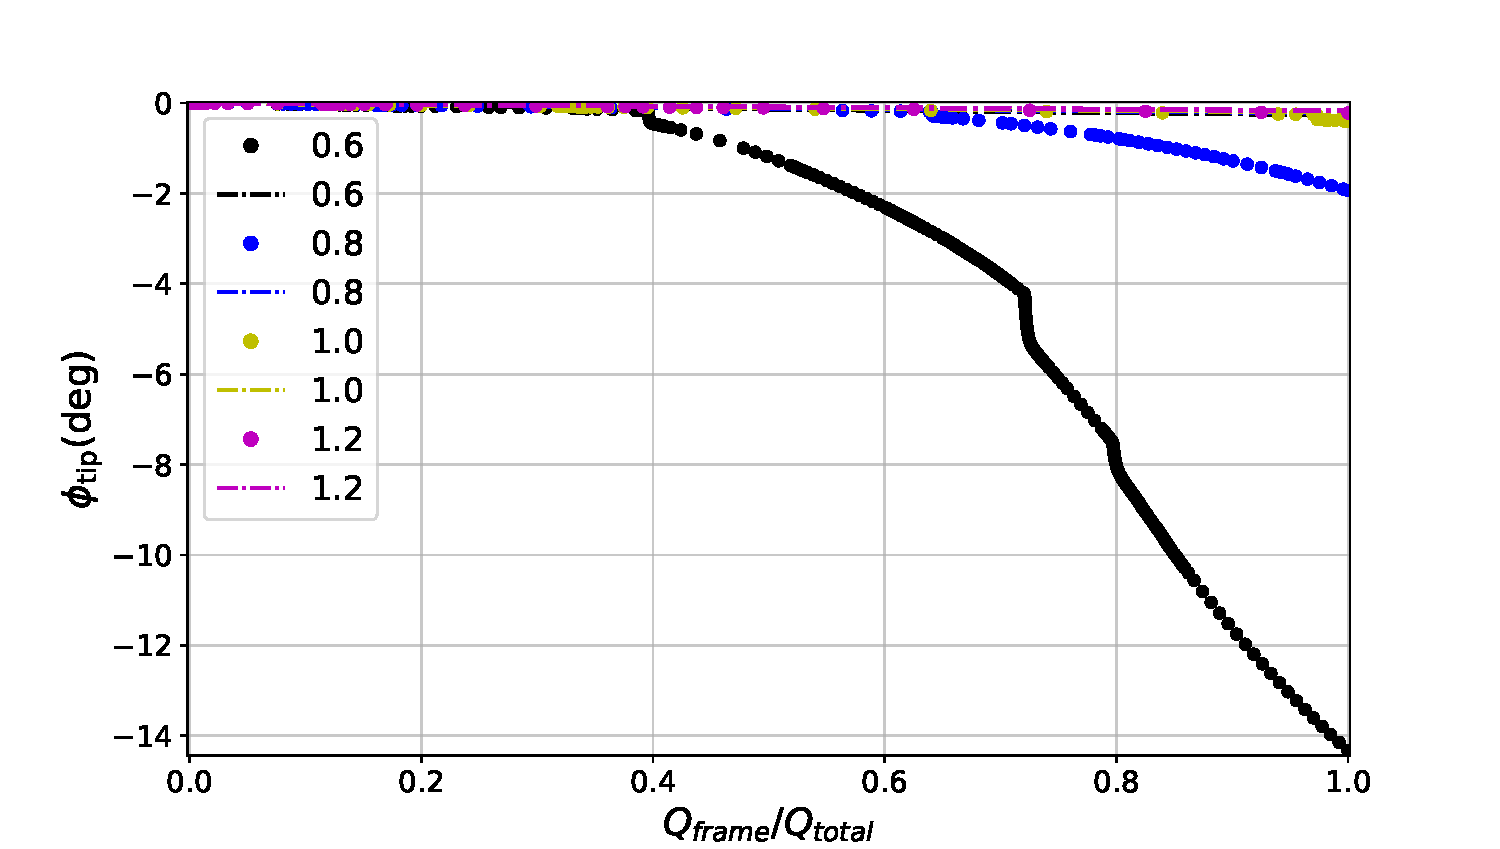
\includegraphics[width=0.8 \textwidth]{../figures/result-sim/cbox/force_displacement-far}
      \caption[Force-displacement curve for various values of the wing-box thickness]{Force-displacement curve for various values of the wing-box thickness \boxt. For all the cases shown, the force applied was located on the upper flange of the tip rib and its magnitude was equal to -800 N.}\label{fig:forceDisplacement-far-Cbox_t}
    \end{figure}

    \begin{figure}[!htpb] %force_displacement-close
      \centering
      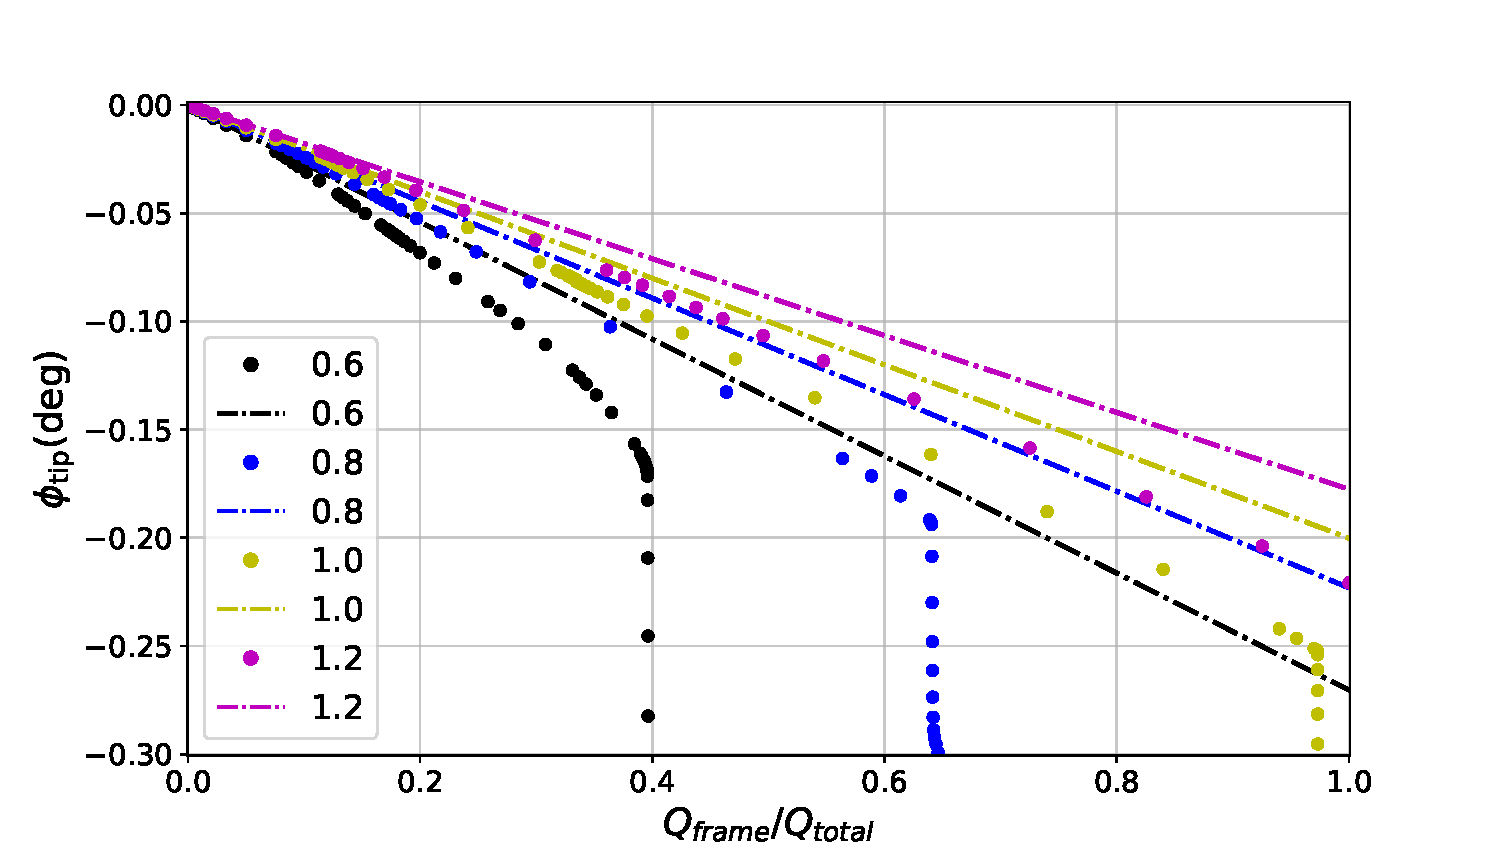
\includegraphics[width=0.8 \textwidth]{../figures/result-sim/cbox/force_displacement-close}
      \caption[Detail of the force-displacement curve for various values of the wing-box thickness]{Detail of the force-displacement curve for various values of the wing-box thickness \boxt. For all the cases shown, the force applied was located on the upper flange of the tip rib and its magnitude was equal to -800 N.}\label{fig:forceDisplacement-close-Cbox_t}
    \end{figure}

    The differences in response for the different cases are also shown the color contour plots provided by Abaqus visualization module. The deformation in the ligaments for \boxt$= 1.2$ mm when buckling occurs is shown in Figure \ref{fig:1coma2-800N-cbox_t} by representing the color contour of the total rotation displacement of the mesh elements. It can be seen buckling does not propagate to other parts of the lattice and it stays where it had appeared on first place, at the first ligaments after the inner rib located further from the root. 

    On the other hand, in Figure \ref{fig:0coma8-800N-cbox_t} the same plot is shown before but not for a value of wing-box thickness of \boxt$= 0.8$ mm. This figure shows the post-buckling state of the structure. In this region, each of the ligaments that had buckled increase its deformation. There are not any new ligaments starting to buckle. It is possible to see that some local deformation has been induced into the upper skin of the wing-box in between the root and the first inner rib. As shown in Table \ref{tab:para_cbox}, for the case $t_{\mathrm{box}} = 0.8$ mm, the point with the maximum vertical is shown to appear close to the root, where $\hat{x}_{v_{\mathrm{max}}} = 0.334$.

    \begin{figure}[!htpb] %force_displacement-close
      \centering
      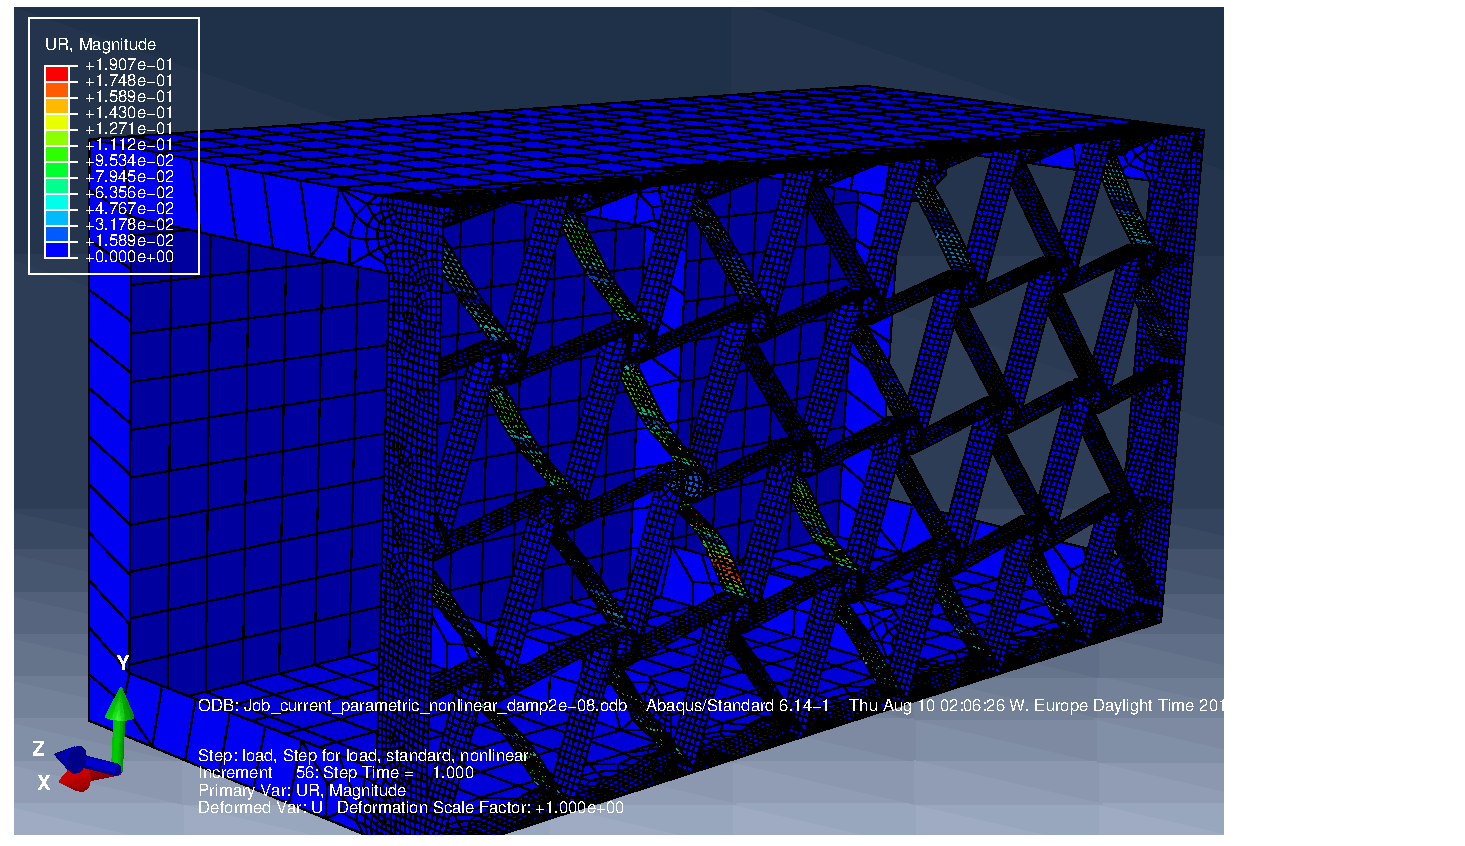
\includegraphics[width=0.8 \textwidth]{../figures/result-sim/cbox/1coma4-800N}
      \caption[Color contour representation of the total angular displacement of the mesh elements on the deformed structure for \boxt$ = 1.2$ mm]{Color contour representation of the total angular displacement of the mesh elements on the deformed structure for \boxt$ = 1.2$ mm. This case is shown after all the prescribed load (800 N) has been applied.}\label{fig:1coma2-800N-cbox_t}
    \end{figure}

    \begin{figure}[!htpb] %force_displacement-close
      \centering
      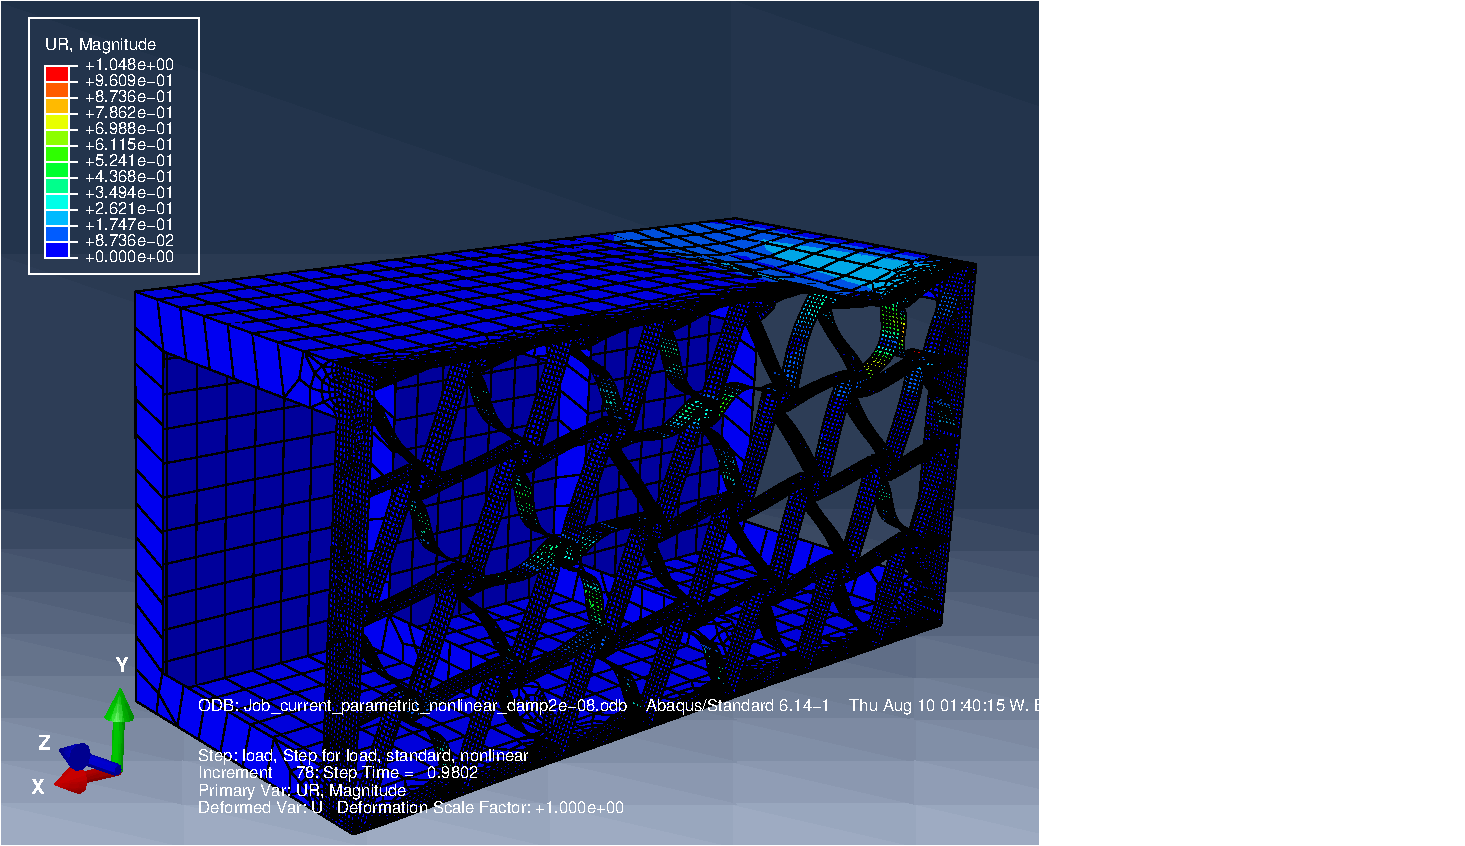
\includegraphics[width=0.8 \textwidth]{../figures/result-sim/cbox/0coma8-800N-2}
      \caption[Color contour representation of the total angular displacement of the mesh elements on the deformed structure for \boxt$ = 0.8$ mm]{Color contour representation of the total angular displacement of the mesh elements on the deformed structure for \boxt$ = 0.8$ mm.}\label{fig:0coma8-800N-cbox_t}
    \end{figure}

    A further study was performed in order to see the relationship between the wing-box thickness and the value of the force applied that induces the structure to collapse. As a result, the plot shown in Figure \ref{fig:force_cbox_t} was produced.

    \begin{figure}[!htpb] %force_displacement-close
      \centering
      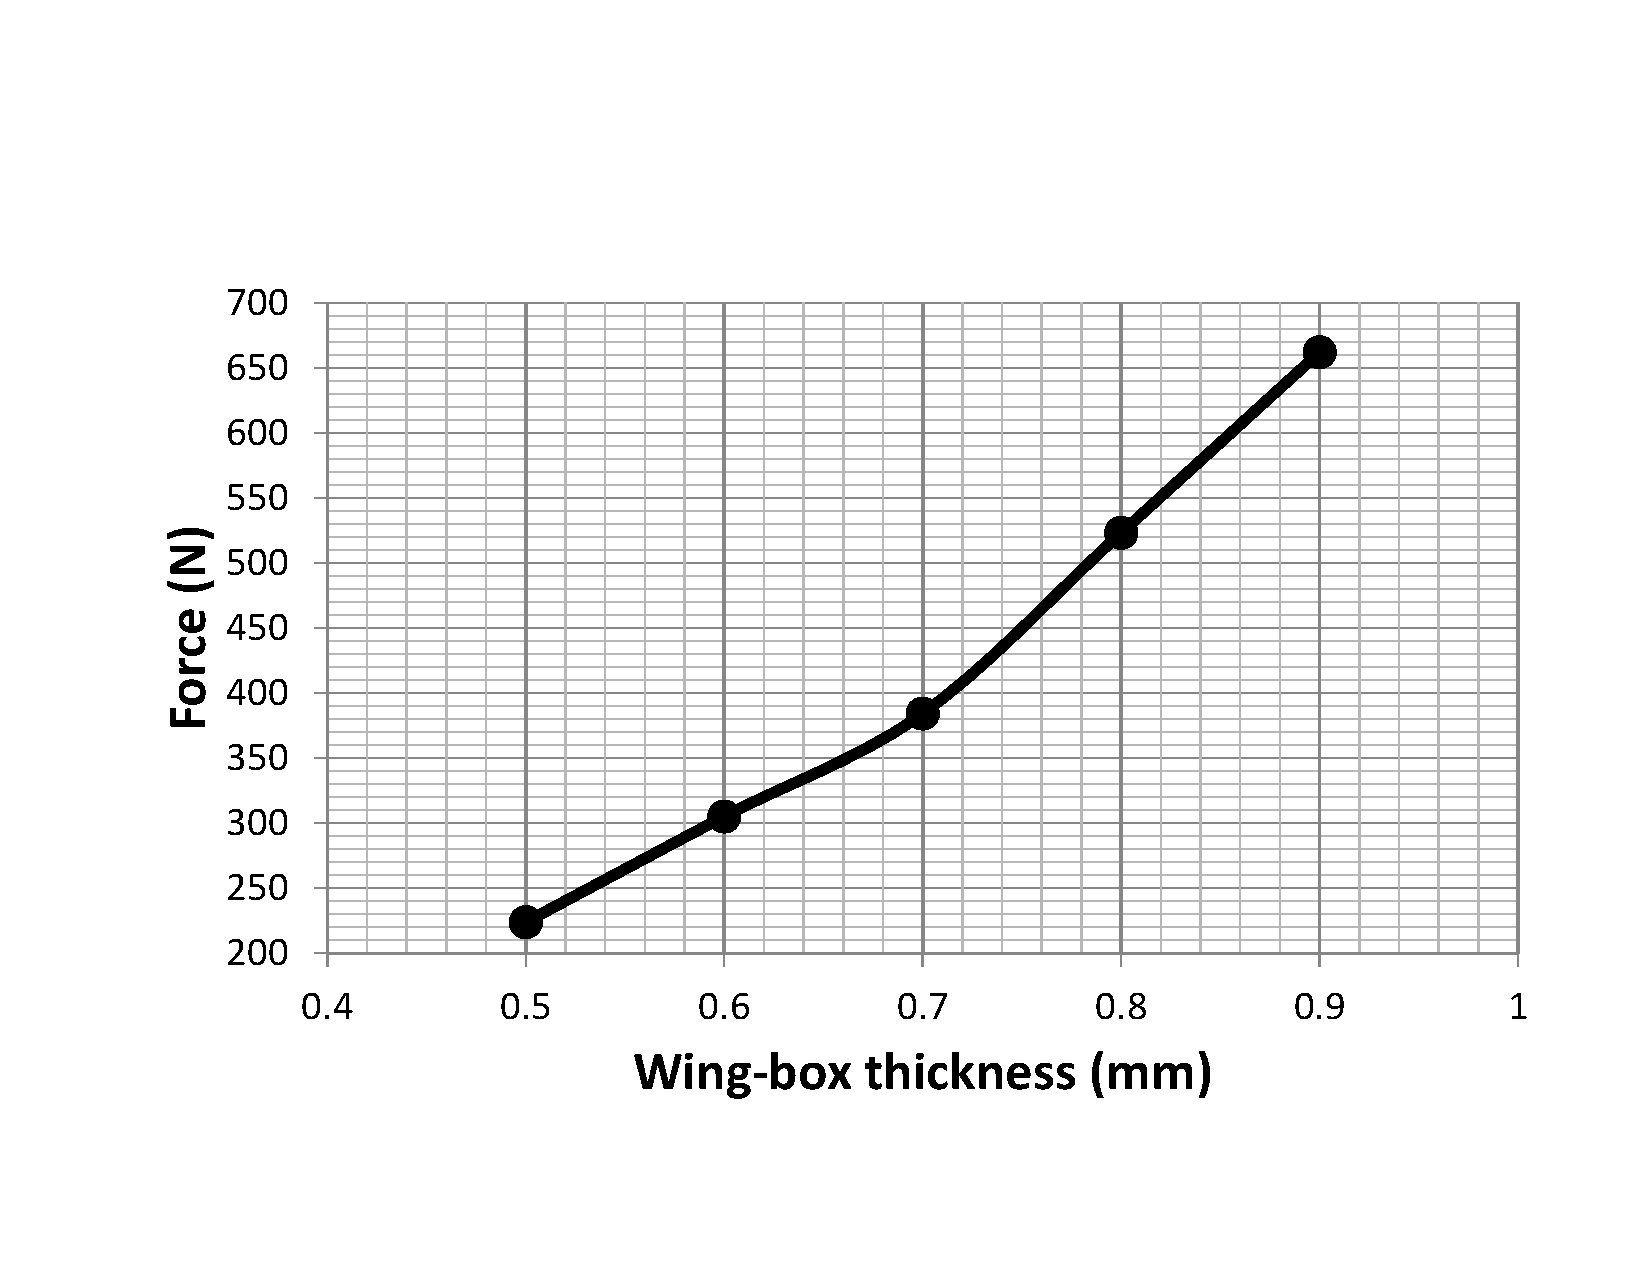
\includegraphics[width=0.8 \textwidth]{../figures/result-sim/cbox/force_cbox_t}
      \caption[Force that induces the structure to collapse as a function of the wing-box thickness]{Force that induces the structure to collapse as a function of the wing-box thickness \boxt.}\label{fig:force_cbox_t}
    \end{figure}

  \clearpage
  \subsection{Number of chiral elements} \label{subsec:MandN_para}
    %
    %   -> For M:
    %       -It was neccessary to increase the load up to 1200N to see the wing-box with $M = 4$ to collapse

    Now the effect of the number of units cells in the transversal direction $M$ and in the spanwise direction $N$ on the structural response are investigated.

    Firstly, the



  \clearpage
  \subsection{Chiral lattice parameters} \label{subsec:chiral_para}

    In the present subsection, different parameters of the chiral lattice structure are varied and its effect of the system response are shown. 

    The parameters chosen 

    \subsubsection{Dimensionless chiral ligament eccentricity $\hat{e}_{\mathrm{chiral}}$}

      The first of this parameters is the ligament eccentricity, in its dimensionless form $\hat{e}_{\mathrm{chiral}}$.
      % \ref{fig:../figures/result-sim/eccen/force_displacement-far}
      % In Figure \ref{fig:../figures/result-sim/eccen/0coma1-700N} it can be seen than the excesive eccentricity of the ligaments keep them from causing the collapse of the structure

    \subsubsection{Chiral node depth $B_{\mathrm{chiral}}$}

      % \ref{fig:../figures/result-sim/B/force_displacement-far}
      % The larger the chiral node depth, the bigger surface on the 
      % The collapse point moves backwards as the $B_{\mathrm{chiral}}$ increases. However, the bigger $B_{\mathrm{chiral}}$, the more abrupt the collapse is.
      % It Figure \ref{fig:../figures/result-sim/B/30_UR1} the rotation $UR_1$ of the mesh elements around the $x$ direction can be seen for the case of \B$= 30$mm at the moment when collapse of the structure ocurrs. The value of this magnitude in this area is approximatelly the double to the corresponding one when \B$= 10$mm which can be seen in Figure \ref{fig:../figures/result-sim/B/10_UR1}

    \subsubsection{Chiral node radius $r_{\mathrm{chiral}}$}

      % Ranges: 7.5, 10, 12.5, 15, 17.5, 20
      % \ref{fig:../figures/result-sim/r/force_displacement-far}
      % For \r = 5, an error in the ligaments is found. There is interference between the mesh elemnents located at different ligaments that are joined at one node.
      % For \r$= 12.5$mm, the buckling ligaments are located at the root, as it can be seen in Figure \ref{fig:../figures/result-sim/r/12coma5-UR}. However, for the case of \r$= 17.5$mm, buckling do not ocurr on the ligaments located at the root but in those located just after the inner rib located closer to the root, with smaller $x$. This explains the characteristic seen in Figure \ref{fig:../figures/result-sim/r/force_displacement-far} for the case of \r$= 17.5$mm which breaks the trend followed by values \r$< 17.5$mm. 

